\documentclass[12pt]{article}

\usepackage{report}

\usepackage[utf8]{inputenc} % allow utf-8 input
\usepackage[T1]{fontenc}    % use 8-bit T1 fonts
\usepackage[colorlinks=true, linkcolor=black, citecolor=blue, urlcolor=blue]{hyperref}       % hyperlinks
\usepackage{url}            % simple URL typesetting
\usepackage{booktabs}       % professional-quality tables
\usepackage{amsfonts}       % blackboard math symbols
\usepackage{nicefrac}       % compact symbols for 1/2, etc.
\usepackage{microtype}      % microtypography
\usepackage{lipsum}		% Can be removed after putting your text content
\usepackage{graphicx}
\usepackage{subcaption}
\usepackage{natbib}
\usepackage{doi}

\usepackage{hyperref}
\usepackage{siunitx}
\usepackage{amsmath}


\usepackage{listings}  % For typesetting code
\usepackage{xcolor}    % For customizing colors

% Define code listing style
\lstset{
    language=C,              % Set the programming language
    basicstyle=\ttfamily,         % Use a monospaced font
    keywordstyle=\color{blue},    % Set keywords to blue
    commentstyle=\color{green},   % Set comments to green
    stringstyle=\color{red},      % Set strings to red
    breaklines=true,              % Enable line breaks
    frame=single,                 % Add a frame around the code
}

\setcitestyle{aysep={,}}



\title{Report of the project for the course of Foundations of High Performance Computing}

\author{Da Vinchie Lisa\\
\AND
Student ID: SM3500574\\
\AND
\AND
\AND
\AND
	Data Science and Scientific Computing\\
\AND
	University of Trieste\\
}

% Uncomment to remove the date
\date{September 2023}

% Uncomment to override  the `A preprint' in the header
\renewcommand{\headeright}{Foundations of High Performance Computing Report}
\renewcommand{\undertitle}{Foundations of High Performance Computing Report}
\renewcommand{\shorttitle}{}


\begin{document}
\maketitle

\newpage
\tableofcontents
\thispagestyle{empty}

\newpage
\thispagestyle{empty}

\begin{abstract}
%	\lipsum[1]
\end{abstract}


% keywords can be removed
%\keywords{First keyword \and Second keyword \and More}


\newpage
\setcounter{page}{1}

\section{Exercise 1: Game of Life}
    \subsection{Introduction}
    In this exercise we were asked to implement Conway's game of life using a hybrid MPI+OpenMP code. The general rules are that:
    \begin{itemize}
        \item Each playground is a matrix of size  $x\,\times\,y$;
        \item Every cell can be either alive (value 1) or dead (value 0);
        \item Each cell becomes or remains alive if 2 or 3 of its neighbours are alive, it dies or continues to be dead otherwise;
        \item The playground must be evolved for $n$ steps and an image of the system must be saved every $s$ steps.
    \end{itemize}

    We have two methods to evolve the playground
    \begin{itemize}
        \item Ordered: evolve one cell after another in row major order. In this case, the status of each cell depends on the previous cells, so this operation is not parallelizable.
        \item Static: evolve each cell based on the information contained in the playground of the previous cycle, that does not change while upgrading.
    \end{itemize}

    For both methods, we are asked to study three kinds of scalability:
    \begin{itemize}
        \item OpenMP scalability: keeping the number of processes fixed to 1, vary the number of threads from 1 up to the maximum number of cores in the socket (12 for THIN, 64 for EPYC); the size of the matrix remains fixed for the whole evolution, in order to have a constant total workload.
        \item Strong scalability: keeping the matrix size fixed, increase the number of processes from 1 up to the maximum number of sockets available, saturating each socket with OpenMP threads.
        \item Weak scalability: increase the number of processes from 1 up to the maximum number of sockets available, like in the Strong scalability, but keeping the workload per process fixed; I achieved that by using rectangular matrices, with one side fixed to 10000 and the other one increasing proportionally with the number of processes, as $10000 \times N_{processes}$.
    \end{itemize}

    The program had to be implemented so that it was divided into two parts:
    \begin{itemize}
        \item Initialisation: initialise a playground of size $x \times y$, specifying its name.
        \item Evolution: read an already existing playground and evolve it, choosing between the static and the ordered method.
    \end{itemize}
    Those options can be selected using inline commands when running the executable file:
    \begin{itemize}
        \item \lstinline{-i} or \lstinline{-r}: initialise a new playground or run an existing one.
        \item \lstinline{-x} and \lstinline{-y}: specify width and height of the matrix; this command is needed only if we are initialising the playground, because if we are running it the program will automatically read the matrix dimensions from the header of the PGM image.
        \item \lstinline{-f <filename>}: if it is used after the \lstinline{-i} command, it specifies the name of the playground that will be created. if it is used after \lstinline{-r}, instead, it indicates the name of the playground that will be evolved.
        \item \lstinline{-e <number>}: if it is followed by 0, the program will use the ordered method for the evolution, while if it is followed by 1 the static evolution will be used; of course, this command is to be used only if the command \lstinline{-r} was previously specified.
        \item \lstinline{-n <number>}: it specifies the number of steps of the evolution.
        \item \lstinline{-s <number>}: it specifies every how many steps a snapshot will be taken.
     \end{itemize}

    \subsubsection{Workload division}
    \label{sect:workload_division}
    In all the sections, the work is divided between processes and threads in the following way:
    \begin{itemize}
        \item First the workload is divided between the processes, giving to each process a specific number of rows to evolve, that in the program is called \lstinline|rows_per_proc|; even though we try to give to each process the same number of rows, that is not always possible, so the value of \lstinline|rows_per_proc| can vary depending on the process.\newline
        So, in each process will be allocated a matrix, called \lstinline|image|, that has the same number of columns as the playground, but a number of rows equal to \lstinline|rows_per_proc + 2|: \lstinline|rows_per_proc| rows are used in the evolution, while the first and the last row are only used to keep the values of the neighbouring cells.\newline
        If we are performing ordered evolution, this matrix will be evolved. If, instead, we are using the static method, this matrix will only be used to calculate the number of live neighbours, and we will need to allocate an auxiliary matrix for each process for the evolution.
        \item If we are performing static evolution, the work to be done on each \lstinline|image| will be split between the OpenMP threads of the process, giving to each thread some cells to evolve in parallel.
    \end{itemize}
    
    
    \subsubsection{Initialisation}
    This part of the code is used to create a random PGM image of the desired dimensions and write it into a pgm file. Since the size of the image can be cery big, i decided to create the matrix in parallel, using a hybrid MPI and OpenMP code.
    
     \subsubsection{Ordered Evolution}
     This kind of evolution is intrinsically serial, since the evolution of every cell depends on the evolution of the previous ones. In order to prove that, I decided to use an MPI code where every process evolves a portion of the martrix and then passes the necessary information to the folllowing process; I did not perform OpenMP scalability for ordered evolution, since dividing this kind of evolution between OpenMP threads is very hard.\newline
     I divided the playground as described in Section \ref{sect:workload_division}; inside the cycle of the generations, I started another cycle on the number of processes: at every cycle, the process receives the first and the last rows of \lstinline|mage| from the previous and following process, evolves the portion of matrix that was assigned to it, then communicates its second and penultimate rows to the previous and following peocesses.\newline
     The communication is done using \lstinline|MPI_Send| and \lstinline|MPI_Recv|, that are two MPI functions that implement blocking communications; that ensures that, every time we are sending a row, the program will not advance until the message is received; in order to make sure that everithing is processed in the correct order, I used many \lstinline|MPI_Barrier| commands.\newline
     To measure the time needed by the program to evolve the palyground, I saved the value of the current time in two places of the program, that are, before and after the for cycle on the number of generations; the difference between those quantities is the time required to evolve the playground, and it is saved in a csv file, that also saves informations about the kind of evolution used, the size of the matrix and the number of processes and threads used.\newline\newline
    
    \subsubsection{Static Evolution}
    This kind of preocess, instead, can be parallelized, since the status of every cell depends on the previous generation; however, exactly because of that, I had to allocate two matrices for each process instead of one:
    \begin{itemize}
    	\item One to keep the status of the cells obtained from the previous cycle, called \lstinline|image|, that has dimension \lstinline|rows_per_proc + 2| $\times$ \lstinline|x| in order to represent the rows that we want to evolve and the two neighboring rows.
    	\item One to write down the result of the evolution, called \lstinline|aux_image|, that has dimension \lstinline|rows_per_proc| $\times$ \lstinline|x|.
   \end{itemize}
    The workload division between the MPI processes is very  similar to the one done in the ordered evolution; after that, I furtherly divided the workload between the OpenMP threads, by assigning some cells of the \lstinline|image| to each one of them for the evolution.\newline
    At the end of each iteration, for each process, the values of the cells of \lstinline|aux_image| are assigned to the cells of \lstinline|image|, from row 1 to row  \lstinline|rows_per_proc|, with a simple for cycle; the rows 0 and \lstinline|rows_per_proc + 2 -1|, instead, must be received from the previous and the following process, and at the same time the rows 1 and \lstinline|rows_per_proc| must be communicated to the same two processes. To achieve that, I used again  \lstinline|MPI_Send| and \lstinline|MPI_Recv|, similarly to what I did in the ordered evolution. This time, however, more than one send and receive operation is performed at the same time, since at the end of the cycle all the \lstinline|image| matrices are fully evolved.\newline
    The time required is measured and saved similarly as in the ordered evolution.
    
    
\section{Results}
	\subsection{Theorethical speed-up}
	The scalability of the program is measured with the speed-up, that is calculated as
	\begin{equation}
		S = \frac{T_{serial}}{T_{parallel}}
	\end{equation}
	
	For the ordered evolution, the theorethical speed-up is always one; actually, we expect it to be a bit less than that in practice, since the communications between processes cause overhead. For the static evolution, instead, there are two cases:
	\begin{itemize}
		\item For the OpenMP and Strong scalability, the theoretical speed up is linear
		\item For the Weak scalability it is constant
	\end{itemize}
	
	In this section, I will show and analyse the results obtained for the two kinds of evolution.
	
    \subsection{OpenMP scalability}
    As we can see in Figure \ref{fig:openmp}, the shape of the measured speed-up is almost linear and very close to the theorethical speed-up, with the THIN nodes giving better results that EPYC; this can be explained with the fact that EPYC nodes have a  larger number of cores per socket: that forces the program to perform more communications between nodes, leading to more communication overhead. Moreover, when using the EPYC nodes, we can observe some fluctuations, to be attribuited to some overhead that we cannot control. The results are pretty similar for all the three matrix sizes used.
    \begin{figure}[h]
    \centering
    \begin{subfigure}[b]{0.4\textwidth}
        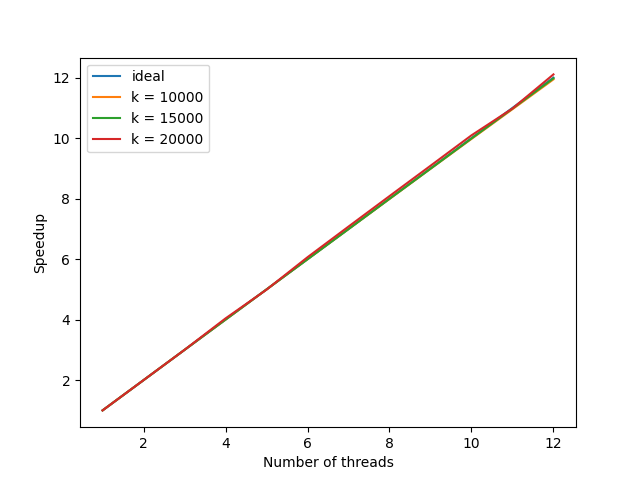
\includegraphics[width = \textwidth]{figs1/OpenMP_scal_THIN.png}
        \caption{Scalability on THIN node}
        \label{fig:openmp_thin}
    \end{subfigure}
    \begin{subfigure}[b]{0.4\textwidth}
        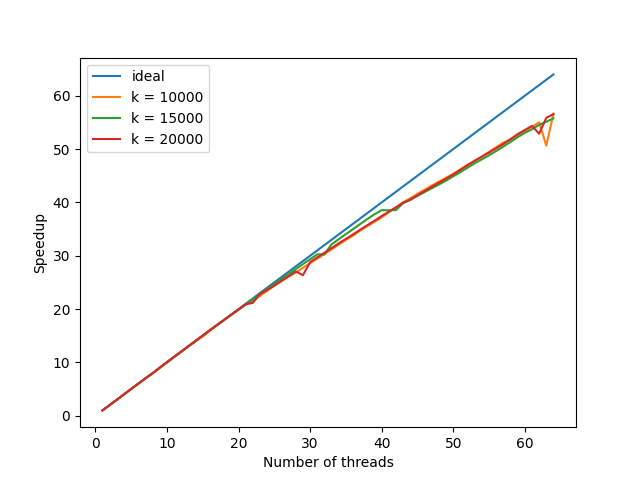
\includegraphics[width = \textwidth]{figs1/OpenMP_scal_EPYC.png}
        \caption{Scalability on EPYC node}
        \label{fig:openmp_epyc}
    \end{subfigure}
    \caption{OpenMP scalability for the static evolution, obtained with different matrix sizes and 50 steps}
    \label{fig:openmp}
    \end{figure}
    
    \subsection{Strong Scalability}
    
    As shown in Figure \ref{fig:strong_static}, the shape of the mesured speed up for the static method has a linear trend; however, it is evident how the measured speed ups are very different from the ideal ones and, contrary to the OpenMP scalability, the greater the matrix size the better the results. This, probably, is explainable with the fact that the required time for communications remains almost the same for all the matrix sizes; as the dimensions of the matrix grow, the time for communication will represent a smaller fraction of the total time, impacting less on the speed-up.\newline
    The communication overhead is probably also responsible for the non perfectly linear trend of the data: as we can observe, the greater the number of processes, the greater the difference between theorethical and measured speed-up. This can be explained with the fact that if we have few processes, we will have few communications between close sockets, since I used the \lstinline|close| affinity policy; a greater number of processes, instead, will lead to more communications, possibly between sockets on different nodes.\newline
    
    \begin{figure}[h]
    \centering
    \begin{subfigure}[b]{0.4\textwidth}
        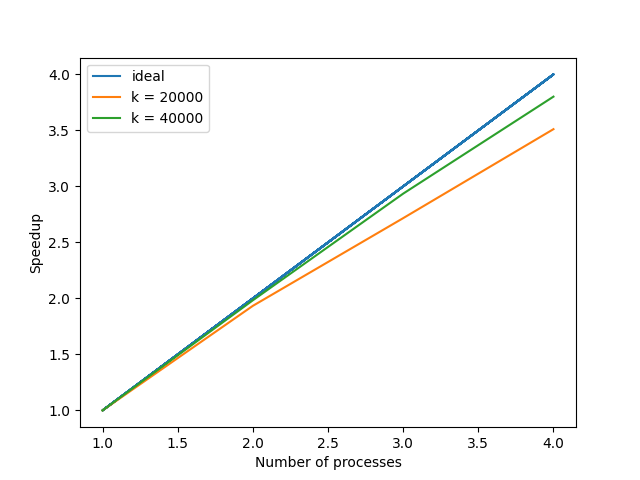
\includegraphics[width = \textwidth]{figs1/Strong_scal_THIN.png}
        \caption{Scalability on THIN node}
        \label{fig:strong_s_thin}
    \end{subfigure}
    \begin{subfigure}[b]{0.4\textwidth}
        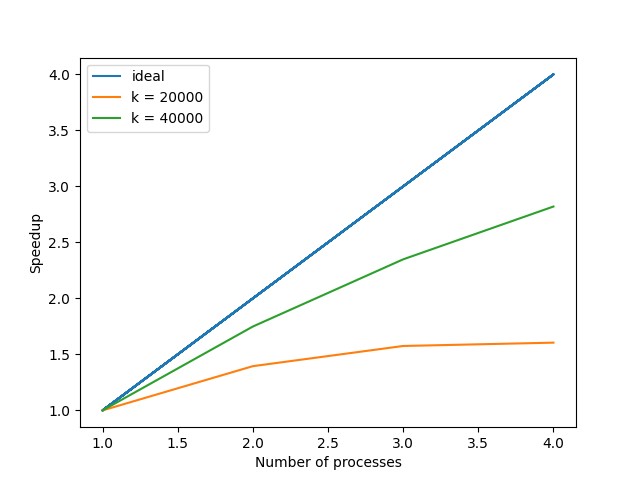
\includegraphics[width = \textwidth]{figs1/Strong_scal_EPYC.png}
        \caption{Scalability on EPYC node}
        \label{fig:strong_s_epyc}
    \end{subfigure}
    \caption{Strong scalability for the static evolution, obtained with different matrix sizes and 50 steps}
    \label{fig:strong_static}
    \end{figure}
    
    For the ordered evolution, instead, the measured results are very close to the theoretical ones, with differences that become visible only when using 3 or 4 processes, as we can see in Figure \ref{fig:strong_ordered}. Those differences can be attribuited, again, to communication overhead.\newline
    In Figure \ref{fig:strong_o_thin}, we can notice that sometimes the measured speed up is slightly greater than one, that is theorethically impossible; this, probably, is due to the fact that, when only one process is present, the communication of the neighboring rows is performed in a different way, since I did not use \lstinline|MPI_Send| \lstinline|MPI_Recv| as in the case of \lstinline|n_procs > 1|; in this case, I communicated the statius of the two rows with a simple for cycle, and that, maybe, is less efficient, leading to an unexpectedly large time for the 1-process case. This may have affected the computation of the speed-up, leading some of them to be greater than one despite the additional communication overhead.\newline
    
     \begin{figure}[h]
    	\centering
    	\begin{subfigure}[b]{0.4\textwidth}
    		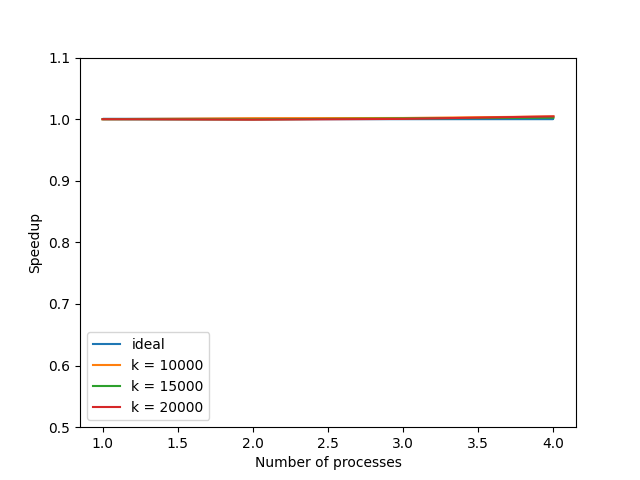
\includegraphics[width = \textwidth]{figs1/Strong_scal_THIN_ordered.png}
    		\caption{Scalability on THIN node}
    		\label{fig:strong_o_thin}
    	\end{subfigure}
    	\begin{subfigure}[b]{0.4\textwidth}
    		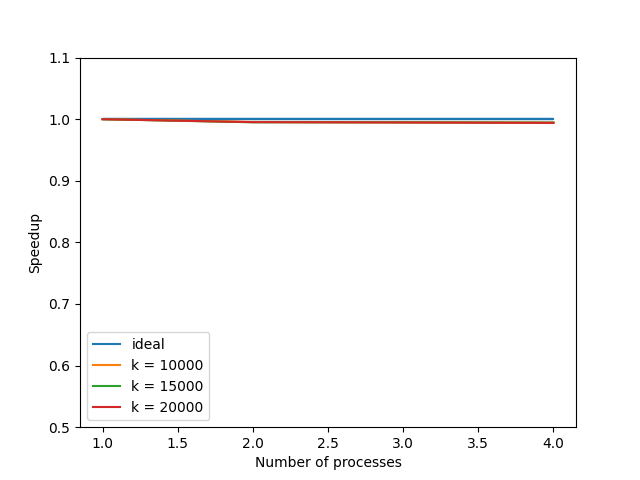
\includegraphics[width = \textwidth]{figs1/Strong_scal_EPYC_ordered.png}
    		\caption{Scalability on EPYC node}
    		\label{fig:strong_o_epyc}
    	\end{subfigure}
    	\caption{Strong scalability for the ordered evolution, obtained with different matrix sizes and 50 steps}
    	\label{fig:strong_ordered}
    \end{figure}
    


    
    \subsection{Weak scalability}
	As I previously said, in the weak scalability the workload per process is constant, so the speed up should be constant and equal to one. As we can see from Figures \ref{fig:weak_static} and \ref{fig:weak_ordered}, the obtained results  are very different from the expected ones, since they present a clear decreasing trend. This can be explained with the fact that, contrary to the strong and openmp scalability, the bigger the matrix size and number of processes, the bigger the fraction of time dedicated to communication.
	
    \begin{figure}[h]
    \centering
    \begin{subfigure}[b]{0.4\textwidth}
        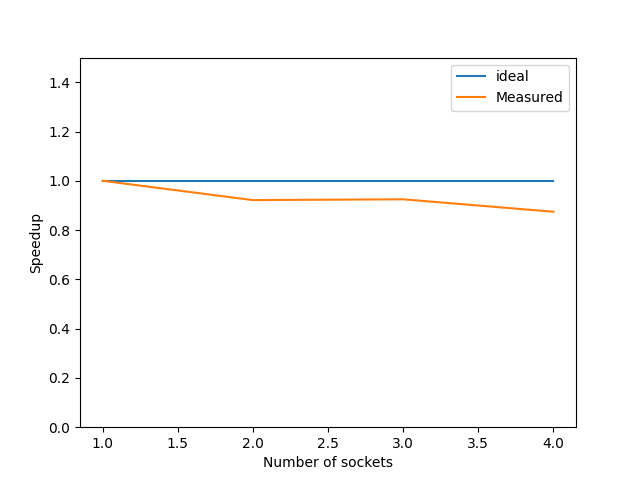
\includegraphics[width = \textwidth]{figs1/Weak_scal_THIN.png}
        \caption{Scalability on THIN node}
        \label{fig:weak_thin}
    \end{subfigure}
		\begin{subfigure}[b]{0.4\textwidth}
		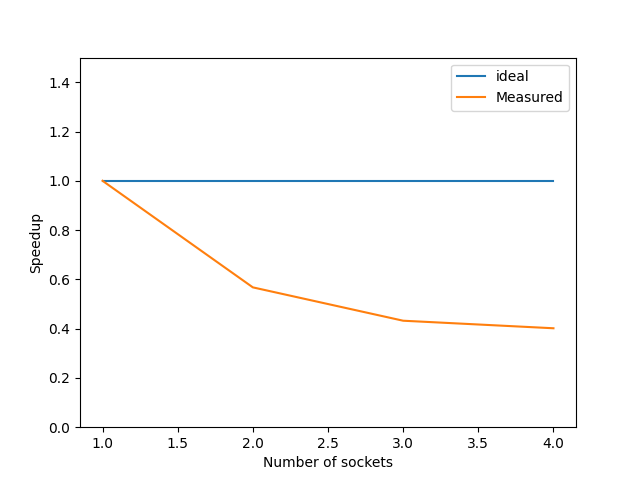
\includegraphics[width = \textwidth]{figs1/Weak_scal_EPYC.png}
		\caption{Scalability on EPYC node}
		\label{fig:weak_epyc}
		\end{subfigure}
    \caption{Weak scalability for the static evolution, keeping the matrix width fixed to 10000 and varying the matrix height and 50 steps}
    \label{fig:weak_static}
    \end{figure}
    
    
      \begin{figure}[h]
    	\centering
    	\begin{subfigure}[b]{0.4\textwidth}
    		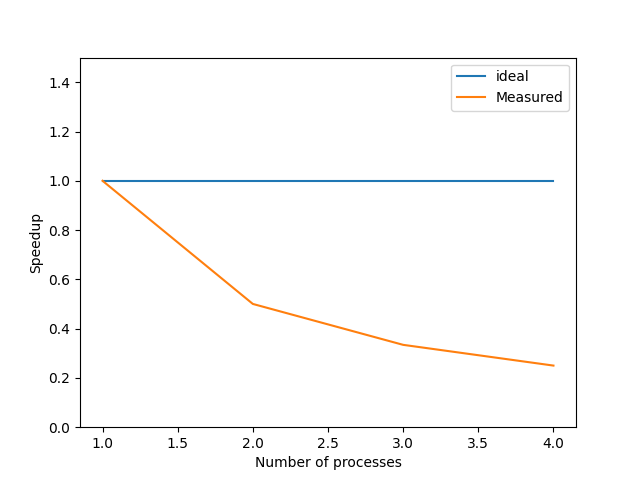
\includegraphics[width = \textwidth]{figs1/Weak_scal_THIN_ordered.png}
    		\caption{Scalability on THIN node}
    		\label{fig:weak_o_thin}
    	\end{subfigure}
    	\begin{subfigure}[b]{0.4\textwidth}
    		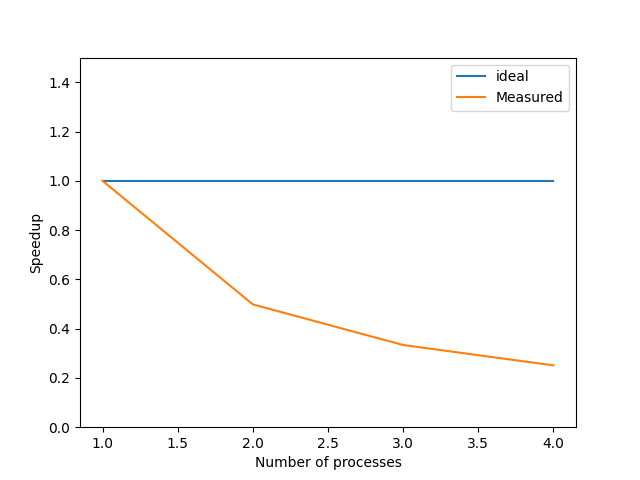
\includegraphics[width = \textwidth]{figs1/Weak_scal_EPYC_ordered.png}
    		\caption{Scalability on EPYC node}
    		\label{fig:weak_o_epyc}
    	\end{subfigure}
    	\caption{Strong scalability for the ordered evolution, obtained with different matrix sizes and 50 steps}
    	\label{fig:weak_ordered}
    \end{figure}



\section{Exercise 2}

    \subsection{Introduction}
%     measure scalability over the size of the matrix at fixed number of cores (12 for thin or 64 for epyc)
% increase the size of matrices size from 2000x2000 to 20000x20000 (single precision) and analyse the scaling of the GEMM calculation for at least MKL and openblas.
% repeat the above point using double precision
% compare with the peak performance of the processor.
% play with different threads allocation policy and discuss the results.
% measure scalability over the number of cores at fixed size. Choose an intermediate size and then:
% increase the number of cores and analyse the scaling of the GEMM calculation for at least MKL and openblas.
% repeat the above point for double precision

    In this exercise, the goal is to compare the performance, measured in Gflops/s, of different math libraries, that are used to perform matrix-matrix multiplication, either in float or double point precision. The three libraries that we are given to compare are
    \begin{itemize}
        \item MKL
        \item OpenBlas
        \item Blis
    \end{itemize}
    The exercise is divided into two tasks, that are:
    \begin{itemize}
        \item Measure how performance changes varying the sizes of the matrices and keeping the number of used cores fixed.
        \item Measure how performance changes varying the number of cores used and keeping the matrices sizes fixed.
    \end{itemize}

    Both tasks can be performed in different conditions, that must be chosen between one of the given options whenever we run the program:
    \begin{itemize}
        \item Library: MKL, OpenBlas or Blis
        \item Partition: THIN or EPYC
        \item Precision: Double or Float
        \item Threads affinity policy: spread or close
        \item Fixed quantity: cores or matrix dimension
    \end{itemize}
    
    \subsection{Implementation}
        In order to perform this exercise, I used three kinds of codes:
        \begin{itemize}
            \item gemm.c: it is the C file that I used to perform the multiplications and save the results. It is a slightly modified version of the dgemm.c code, that was given to us along with the assignment, where I added the possibility to save the obtained time and performance results in a csv file.\newline
            The program accepts command line arguments to specify:
            \begin{itemize}
                \item The library to use, to be chosen between \textbf{MKL}, \textbf{OPENBLAS} and \textbf{BLIS}.
                \item The desired precision, to be chosen between \textbf{USE\_DOUBLE} and \textbf{USE\_FLOAT}.
                \item If we want to save the results in a csv file, using the \textbf{SAVE\_RESULTS} flag.
                \item The dimensions of the two matrices that we want to multiply. Since the number of rows of the first matrix must be equal to the number of columns of the second one, we only have three positional arguments; personally, I decided to use only square matrices.
            \end{itemize}
            Since this file is used for both tasks, there is only one version of it, that is in the exercise1 folder
            \item Makefile: it is used to compile and run the gemm.c program, for all the three libraries; using the phony targets \textbf{float} and \textbf{double}, we can decide whether we want to run the program with float or double precision.
            \item Sbatch files: I used one sbatch file for every possible combination of fixed quantity and partition, that is, four sbatch files in total, that are used in order to:
            \begin{itemize}
                \item Specify the partition that we intend to use and allocate the required number of cores
                \item Load the modules
                \item Specify the thread affinity policy
                \item Call the Makefile in order to compile the C file
                \item Use a for cycle in order to run the executable files for different matrix dimensions or cores
            \end{itemize}
        \end{itemize} 
    
    \subsection{Results}
        \subsection{Theoretical peak performance}
        The theoretical peak performances for each core can be calculated either as
        \begin{equation}
            TPP = \text{cores} \times \text{frequency} \times \text{flops per cycle}
        \end{equation}
        or by dividing the peak performance of the whole node for the number of cores of the node, depending on what data we have.\newline
        For the EPYC nodes I used the first method, since all the information needed is reported \href{https://github.com/Foundations-of-HPC/Foundations_of_HPC_2022/blob/main/Basic/Benchmarking/running-HPL/hpl-on-epyc.md}{here};
        using those data I calculated that the theoretical peak performance for each core is
        \begin{equation}
        \begin{aligned}
            TPP_{EPYC}^{double} &= \SI{2.6}{GHz} \times \SI{16}{Flops/cycle} = \SI{41.60}{GFlops/s}\\
            TPP_{EPYC}^{float} &= 2 \times TPP_{EPYC}^{double} = \SI{83.20}{Gflops/cycle}
        \end{aligned}
        \end{equation}
        In the case of THIN nodes, instead, I couldn't find any information about the frequency or the flops per cycle, but the  \href{https://raw.githubusercontent.com/Foundations-of-HPC/Foundations_of_HPC_2022/main/Basic/Intro/lecture02-HPC-hardware.pdf}{course slides} reported the theoretical peak performance for the whole node and the number of cores per node, so I used the second strategy:
        \begin{equation}
        \begin{aligned}
            TPP_{THIN}^{double} &= \frac{\SI{1997}{GFlops/s}}{\SI{24}{cores}} = \SI{83.21}{GFlops/s}\\
            TPP_{THIN}^{float} &= 2 \times TPP_{THIN}^{double} = \SI{166.42}{GFlops/s}
        \end{aligned}
        \label{eq:TPP}
        \end{equation}
        
        
        \subsubsection{Size scalability}
        In the following figures I examine the relation between performance, measured in Gflops, and matrix dimension, keeping the number of cores constant.\newline
        As required in the assignment, in the this case I fixed the number of cores to 12 for the THIN nodes and to 64 for the EPYC nodes; the matrix dimensions, instead, varied from 2000 to 20000, using steps of 500; for each matrix dimension, the programs were run five times.

        \begin{figure}[h]
            \centering
            \begin{subfigure}[b]{0.4\textwidth}
                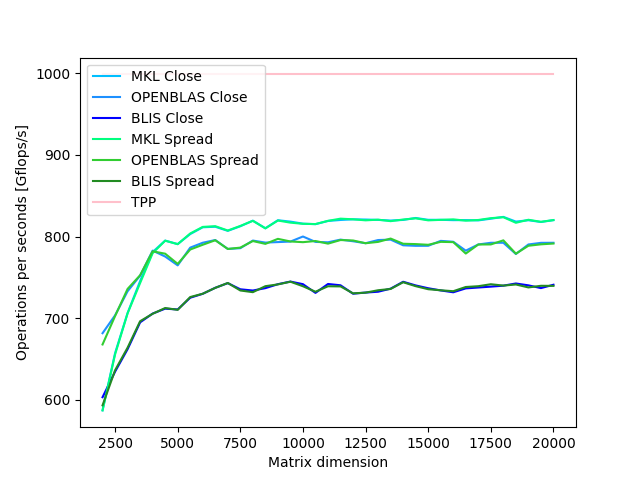
\includegraphics[width = \textwidth]{figs2/fixed_cores_THIN_d.png}
                \caption{THIN node and double precision}
                \label{fig:fixed_cores_thin_d}
            \end{subfigure}
            \begin{subfigure}[b]{0.4\textwidth}
                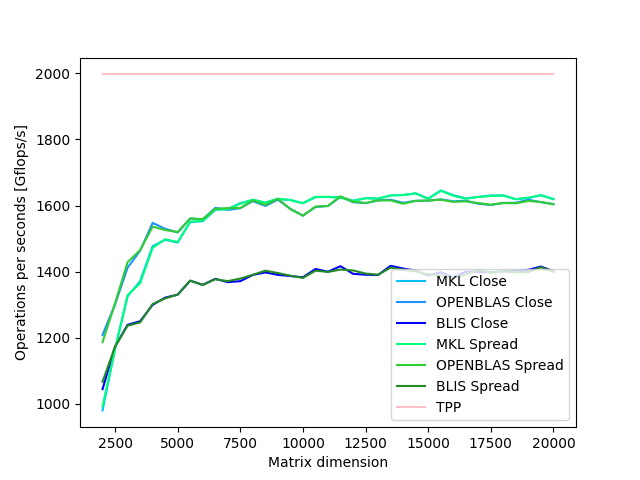
\includegraphics[width = \textwidth]{figs2/fixed_cores_THIN_f.png}
                \caption{THIN node and float precision}
                \label{fig:fixed_cores_thin_f}
            \end{subfigure}
            \begin{subfigure}[b]{0.4\textwidth}
                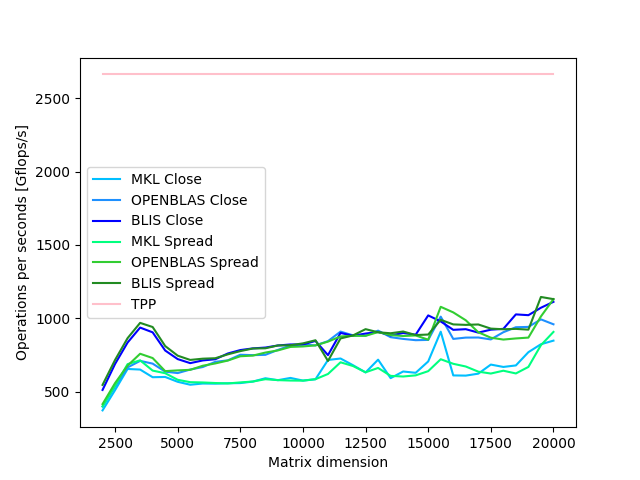
\includegraphics[width = \textwidth]{figs2/fixed_cores_EPYC_d.png}
                \caption{EPYC node and double precision}
                \label{fig:fixed_cores_epyc_d}
            \end{subfigure}
            \begin{subfigure}[b]{0.4\textwidth}
                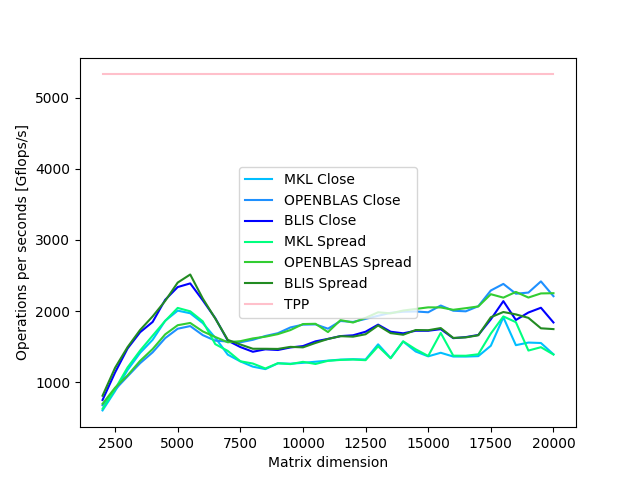
\includegraphics[width = \textwidth]{figs2/fixed_cores_EPYC_f.png}
                \caption{EPYC node and float precision}
                \label{fig:fixed_cores_epyc_f}
            \end{subfigure}
            \caption{Results obtained fixing the number of cores and changing the size of the matrices}
            \label{fig:fixed_cores}
        \end{figure}

        Ideally, the performance should be constant, since the number of cores is fixed; the theoretical peak performances for each kind of node and precision can be calculated by multiplying the corresponding TPP per core, calculated in Equation \eqref{eq:TPP}, for the number of cores used.\newline
        As we can see from Figure \ref{fig:fixed_cores}, the measured performance is much lower than the theoretical one, with the THIN nodes being closer to TPP than the EPYC ones. The thread affinity does not affect the performance since we are using just one socket and all its cores, so the way that we use to choose them does not change the final result.\newline
        When using THIN nodes, the library with the best performance is MKL, while the one with the worst performance is BLIS; when using EPYC nodes the roles are reversed and the differences between the three libraries are smaller.\newline
        We can also notice that the graphs of the two nodes present two different trends: when using the THIN nodes, the performance increases until the matrix dimension is more or less 5000, then it stabilises. When using the EPYC nodes, instead, the performance increases rapidly for small matrix dimensions,reaching a peak between 2500 and 5000, then it decreases rapidly and increases slightly for greater matrix dimensions.\newline
        This can be explained with the different number of cores of the two kinds of node: THIN nodes only have 12 cores, while EPYC nodes have 64 cores.

        \subsubsection{Fixed matrix dimension}
            In the following figures I examine the relation between performance, measured in Gflops, and number of cores, keeping the dimension of the two matrices constant.\newline
            As we can see in Figure \ref{fig:fixed_matrix}, all the three libraries perform way better on THIN nodes rather than on the EPYC ones; as we can see from figures \ref{fig:fixed_matrix_epyc_d} and \ref{fig:fixed_matrix_epyc_f}, the measured performance is pretty close to the theoretical one when the number of threads is less than 10, then the performance stabilizes and the difference becomes more visible, with not significant differences between the three libraries. Moreover, since we can observe a slow but constant increase in the performance, it is possible that the matrix size used, 10000 is too small to fully exploit parallelization, and that bigger sizes could lead to better results.

         \begin{figure}[h]
            \centering
            \begin{subfigure}[b]{0.4\textwidth}
                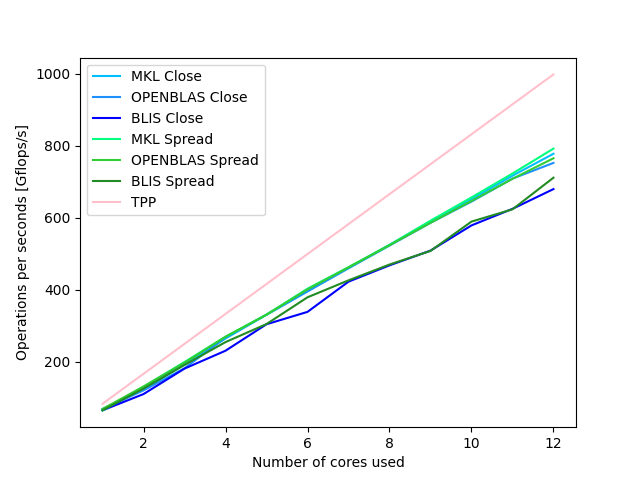
\includegraphics[width = \textwidth]{figs2/fixed_matrix_THIN_d.png}
                \caption{THIN node and double precision}
                \label{fig:fixed_matrix_thin_d}
            \end{subfigure}
            \begin{subfigure}[b]{0.4\textwidth}
                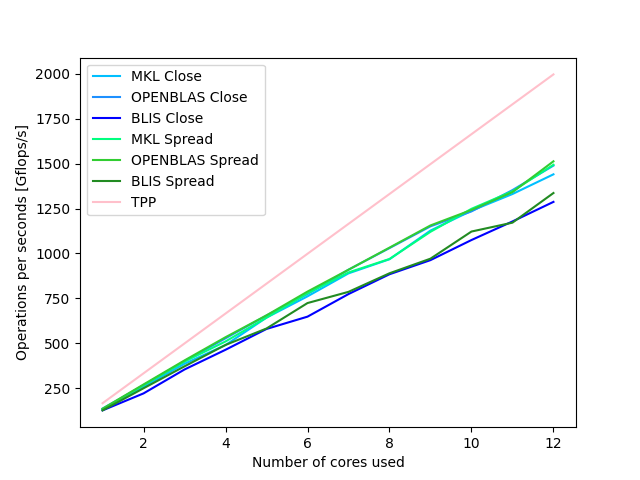
\includegraphics[width = \textwidth]{figs2/fixed_matrix_THIN_f.png}
                \caption{THIN node and float precision}
                \label{fig:fixed_matrix_thin_f}
            \end{subfigure}
            \begin{subfigure}[b]{0.4\textwidth}
                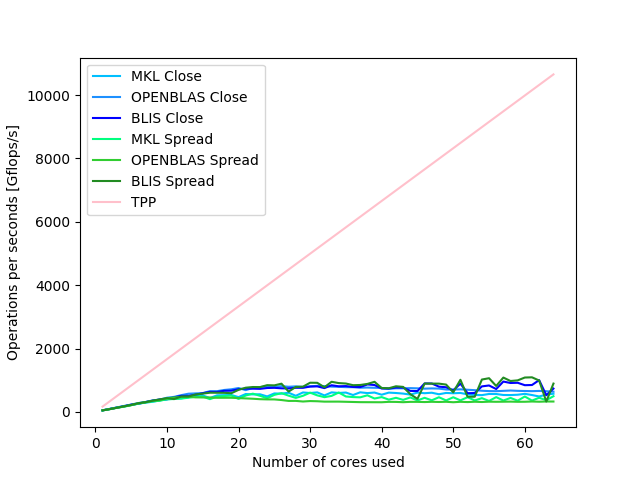
\includegraphics[width = \textwidth]{figs2/fixed_matrix_EPYC_d.png}
                \caption{EPYC node and double precision}
                \label{fig:fixed_matrix_epyc_d}
            \end{subfigure}
            \begin{subfigure}[b]{0.4\textwidth}
                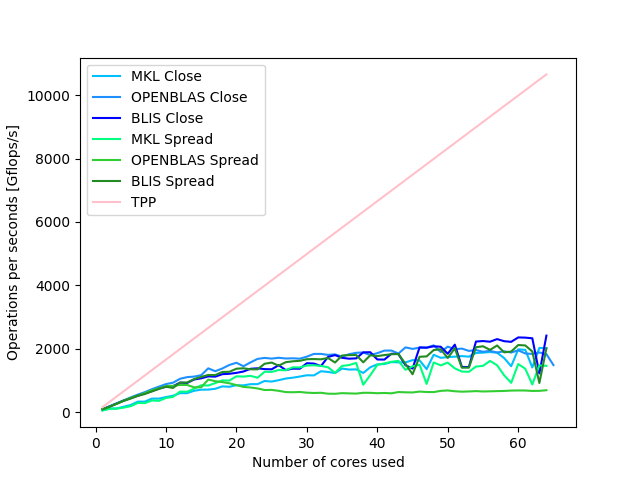
\includegraphics[width = \textwidth]{figs2/fixed_matrix_EPYC_f.png}
                \caption{EPYC node and float precision}
                \label{fig:fixed_matrix_epyc_f}
            \end{subfigure}
            \caption{Results obtained fixing the size of the matrices and changing the number of cores}
            \label{fig:fixed_matrix}
        \end{figure}

		In conclusion, we can say that the three libraries are unable to fully exploit all the cores; this, maybe, is also due to the matrix sizes used, that may be to small to efficiently parallelize the workload.


\end{document}
